\section{Results}

Table detection exhibits very high accuracy, in particular for each initial frame of each video four corner points are consistently identified across the dataset, the assumption that we made is that the camera does not move during a single clip so once the table is detected in the first frame we can use that information for all the frames of the same video.
In contrast, ball detection is influenced by k-means clustering. To achieve consistent and satisfactory results, a fixed random seed is incorporated into the code. This method results in an average mAP of 0.51 for the dataset.

\subsection{Quantitative results}
The \textit{computePerformance} executable calculates the detection and segmentation performance across the dataset.
\begin{table}
	\centering
    \begin{tabular}{|c|c|}
        \hline
        mAP & mIoU \\
        \hline
        0.51 & 0.69 \\
        \hline
    \end{tabular}
    \caption{Performance of the detection and segmentation}
    \label{tab: performance}
\end{table}
While the method successfully detects tables, backgrounds, and both white and black balls with high Intersection
over Union (IoU), it struggles with solid and striped balls due to inaccurate classification.
This leads to a lower overall mean Average Precision (mAP) that is focused only on balls,
but a good mean Intersection over Union (mIoU) because the background and playing field are identified well.

\subsection{Qualitative results}
Below some qualitative results are presented.
\begin{figure}[H]
    \centering
    \begin{subfigure}[b]{0.4\textwidth}
        \centering
        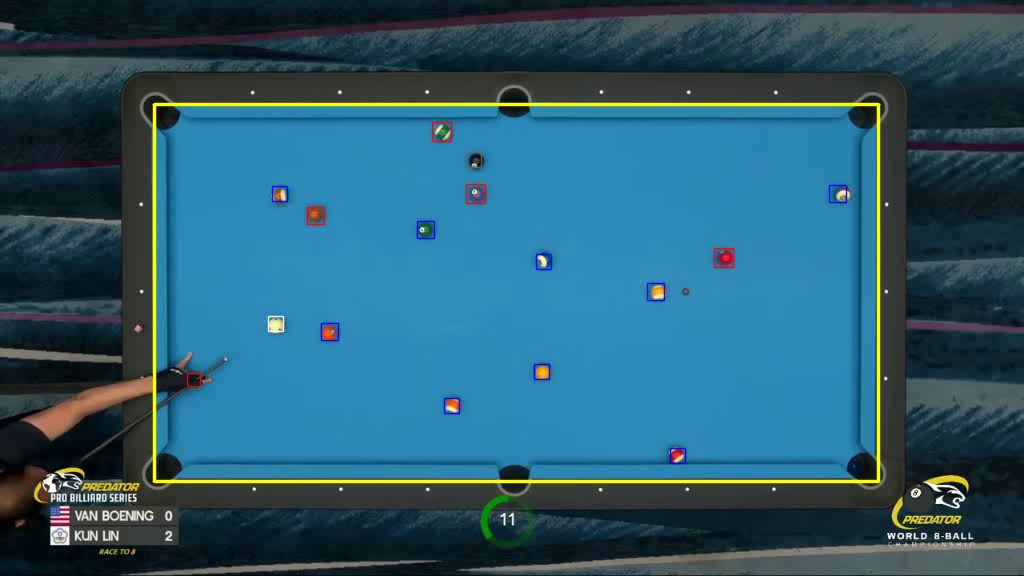
\includegraphics[width=\textwidth]{images/Detection/game1_clip1_detected_balls_first_frame.jpg}
        \caption{Detection game1 clip1 first frame}
        \label{fig: game1_clip1_first_frame_detected}
    \end{subfigure}
    \begin{subfigure}[b]{0.4\textwidth}
        \centering
        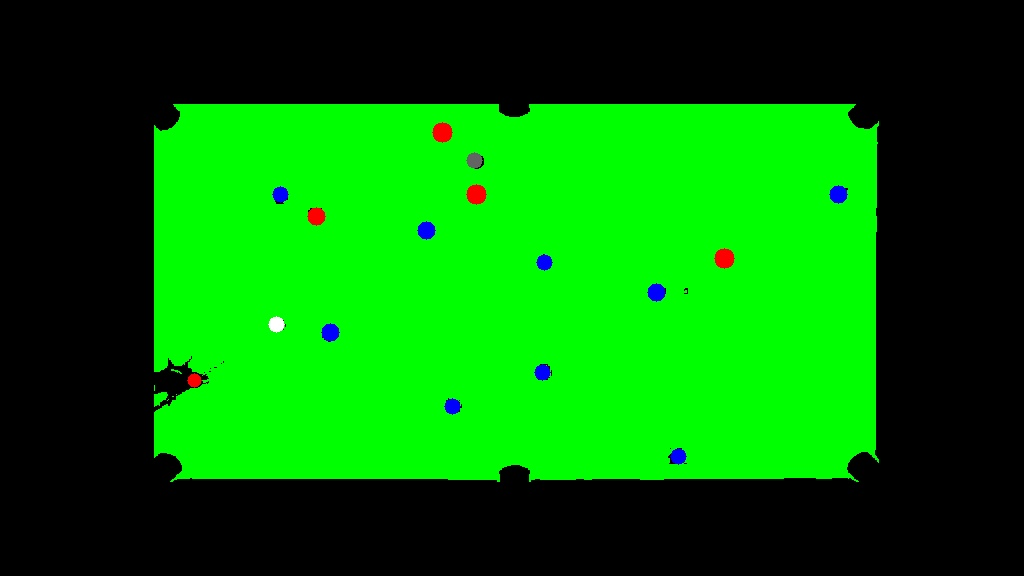
\includegraphics[width=\textwidth]{images/Segmentation/game1_clip1_segmented_balls_first_frame.jpg}
        \caption{Segmentation game1 clip1 first frame}
		\label{fig: game1_clip1_first_frame_segmented}
    \end{subfigure}
	\caption{game1 clip1 first frame}
\end{figure}


\begin{figure}[H]
    \centering
    \begin{subfigure}[b]{0.4\textwidth}
        \centering
        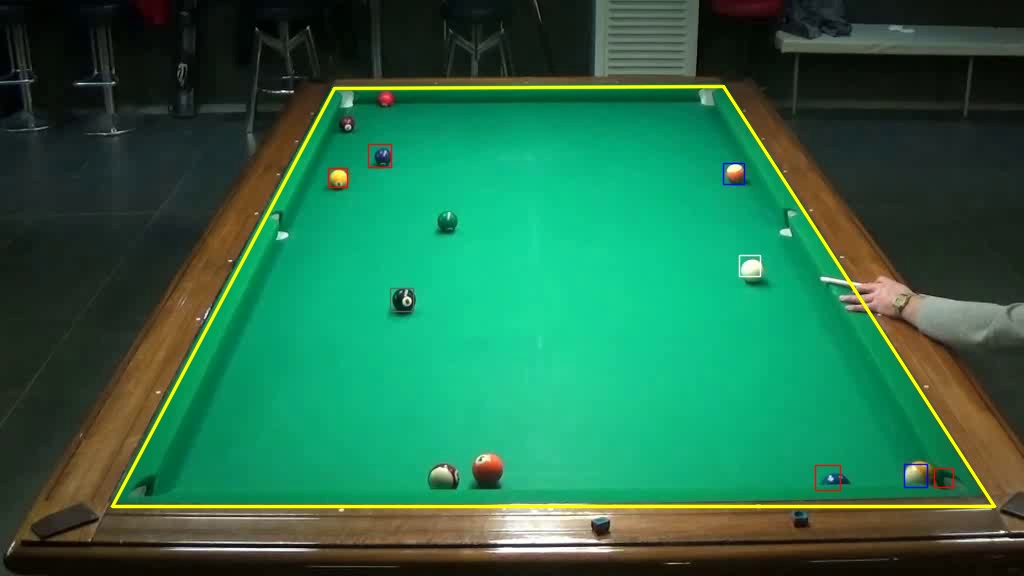
\includegraphics[width=\textwidth]{images/Detection/game2_clip1_detected_balls_first_frame.jpg}
        \caption{Detection game2 clip1 first frame}
        \label{fig: game2_clip1_first_frame_detected}
    \end{subfigure}
    \begin{subfigure}[b]{0.4\textwidth}
        \centering
        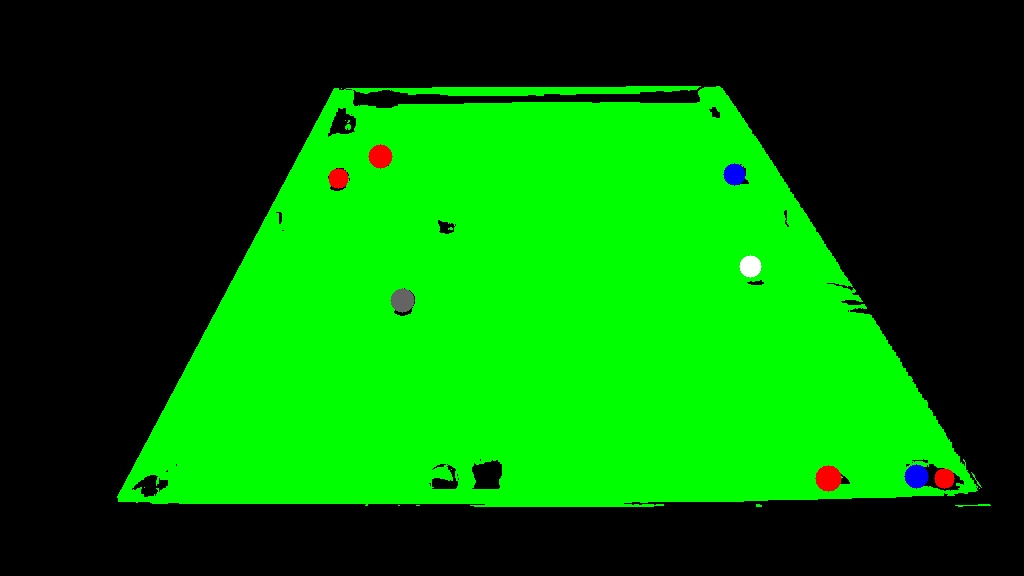
\includegraphics[width=\textwidth]{images/Segmentation/game2_clip1_segmented_balls_first_frame.jpg}
        \caption{Segmentation game2 clip1 first frame}
		\label{fig: game2_clip1_first_frame_segmented}
    \end{subfigure}
	\caption{game2 clip1 first frame}
\end{figure}

\begin{figure}[H]
    \centering
    \begin{subfigure}[b]{0.4\textwidth}
        \centering
        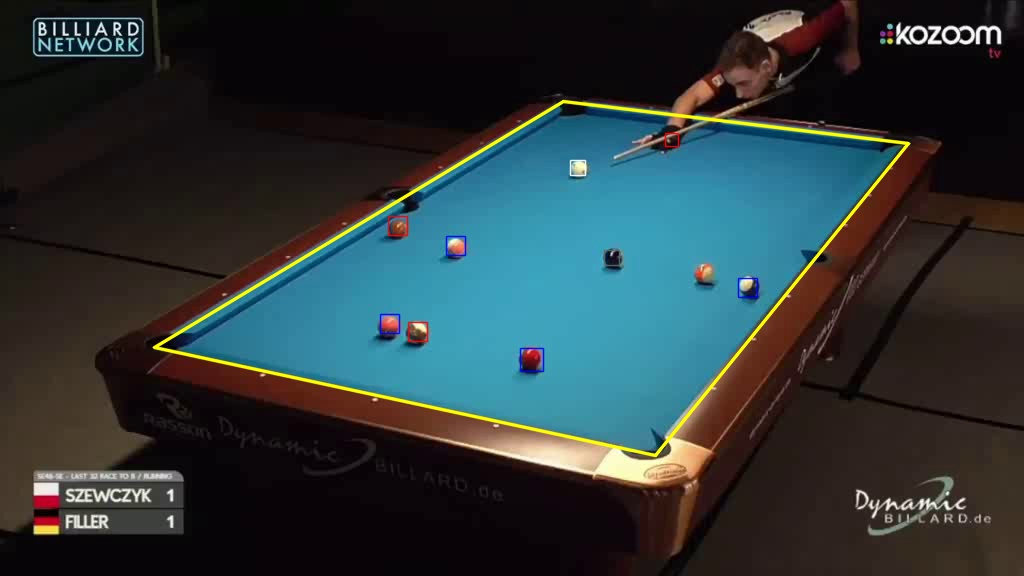
\includegraphics[width=\textwidth]{images/Detection/game3_clip1_detected_balls_first_frame.jpg}
        \caption{Detection game3 clip1 first frame}
        \label{fig: game3_clip1_first_frame_detected}
    \end{subfigure}
    \begin{subfigure}[b]{0.4\textwidth}
        \centering
        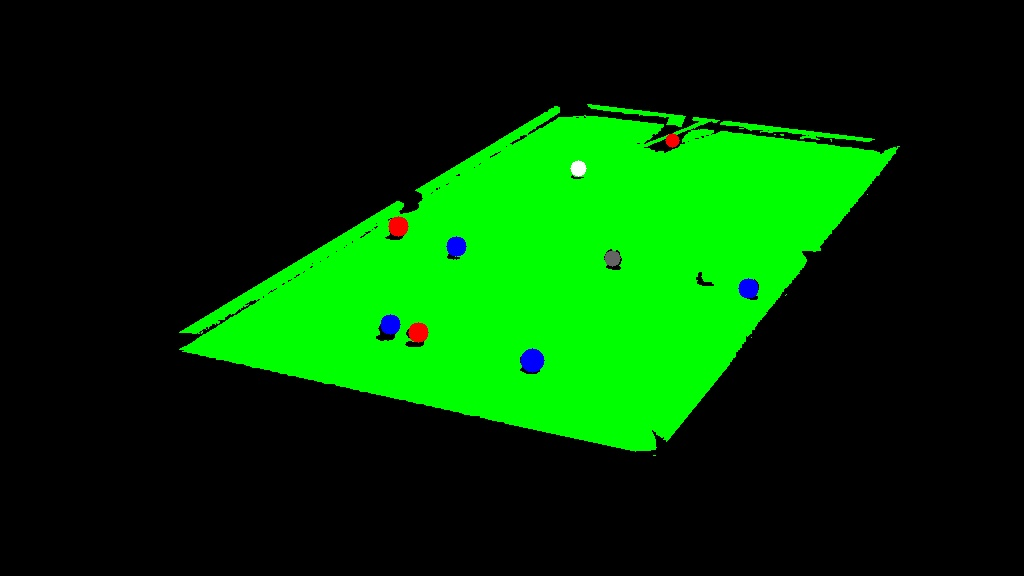
\includegraphics[width=\textwidth]{images/Segmentation/game3_clip1_segmented_balls_first_frame.jpg}
        \caption{Segmentation game3 clip1 first frame}
		\label{fig: game3_clip1_first_frame_segmented}
    \end{subfigure}
	\caption{game3 clip1 first frame}
\end{figure}

\begin{figure}[H]
    \centering
    \begin{subfigure}[b]{0.4\textwidth}
        \centering
        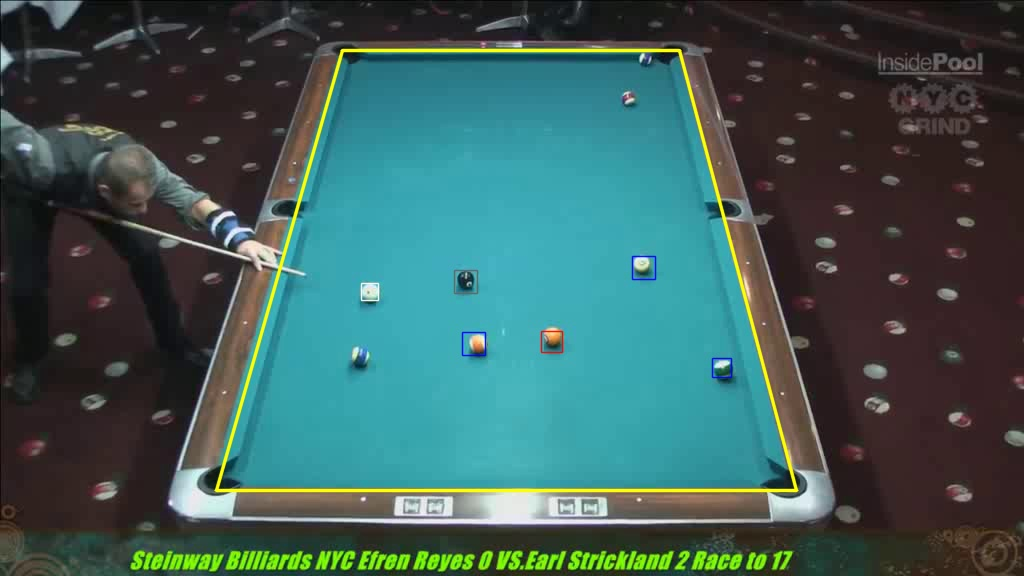
\includegraphics[width=\textwidth]{images/Detection/game4_clip1_detected_balls_first_frame.jpg}
        \caption{Detection game4 clip1 first frame}
        \label{fig: game4_clip1_first_frame_detected}
    \end{subfigure}
    \begin{subfigure}[b]{0.4\textwidth}
        \centering
        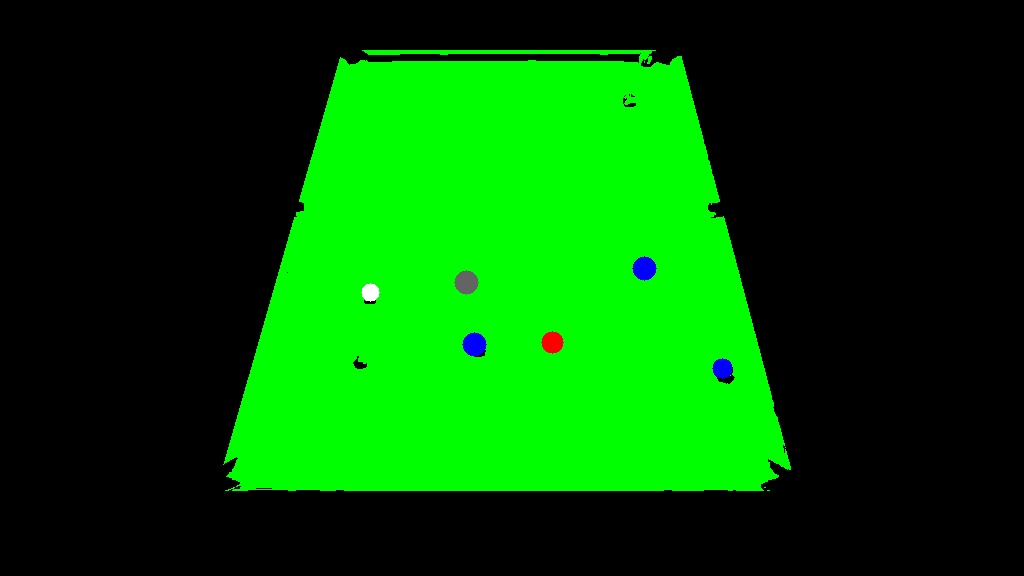
\includegraphics[width=\textwidth]{images/Segmentation/game4_clip1_segmented_balls_first_frame.jpg}
        \caption{Segmentation game4 clip1 first frame}
		\label{fig: game4_clip1_first_frame_segmented}
    \end{subfigure}
	\caption{game4 clip1 first frame}
\end{figure}
